\chapter{Contribution}
\label{chapter_3}

In this internship, we follow the direction of using spatial filtering to remove noise from images of SWARMS project. The studied methods include  Median Filter, Average Filter, Gaussian Filter and Wiener Filter. The following sections will present in detail each of these methods.

%%
\section{Median Filter}

Median filter is a spatial filter which applies to a neighborhood (local method). It is a non-linear filter which replaces each pixel value in the image with the median of its neighbors and itself. In this method, the heavy task is the calculation of median for each neighbor area. Specifically, for calculating each median, we first order all pixel values in the neighborhood area, then replace the considered pixel with pixel value in the middle of the sorted list. If the neighborhood area contains an even number of pixels, median will be taken as the two middle pixel values. Table~\ref{tab:median_filter} shows an example to calculate median of a 5$\times$5 image pixels having filter kernel of size 3$\times$3. From this table, firstly the considered pixel is $156$ in red color; secondly, the neighborhood pixels of size 3$\times$3 are 123 121 223 223 156 178 125 211 178. By sorting these values, we have sorted pixel values are 121 123 125 156 178 178 211 223 223. Thirdly, the median value should be 178 and be the representative of its surrounding pixels.

%%%
\begin{table*}[tb]
	\caption{Example of median computation} 
	\label{tab:median_filter}
	\begin{center}
		\begin{tabular}{|c|c|c|c|c|}
		\hline 
		234 & 147 & 225 & 214 & 134 \\ 
		\hline 
		231 & \textcolor{blue}{123} & \textcolor{blue}{121} & \textcolor{blue}{223} & 189 \\ 
		\hline 
		124 & \textcolor{blue}{223} & \textcolor{red}{156} & \textcolor{blue}{178} & 196 \\ 
		\hline 
		219 & \textcolor{blue}{125} & \textcolor{blue}{211} & \textcolor{blue}{178} & 124 \\ 
		\hline 
		210 & 185 & 221 & 189 & 134 \\ 
		\hline 
		\end{tabular}
	\end{center}

	\begin{center}
		\begin{tabular}{|c|c|c|c|c|}
		\hline 
		\textcolor{white}{234} & \textcolor{white}{234} & \textcolor{white}{234} & \textcolor{white}{234} & \textcolor{white}{234} \\ 
		\hline 
		\textcolor{white}{234} & \textcolor{white}{234} & \textcolor{white}{234} & \textcolor{white}{234} & \textcolor{white}{234} \\ 
		\hline 
		\textcolor{white}{234} & \textcolor{white}{223} & \textcolor{red}{178} & \textcolor{white}{178} & \textcolor{white}{234} \\ 
		\hline 
		\textcolor{white}{234} & \textcolor{white}{234} & \textcolor{white}{234} & \textcolor{white}{234} & \textcolor{white}{234} \\ 
		\hline 
		\textcolor{white}{234} & \textcolor{white}{234} & \textcolor{white}{234} & \textcolor{white}{234} & \textcolor{white}{234} \\ 
		\hline 
		\end{tabular}
	\end{center}
\end{table*}

%%%		
\begin{figure}[!ht]		
	\centering
	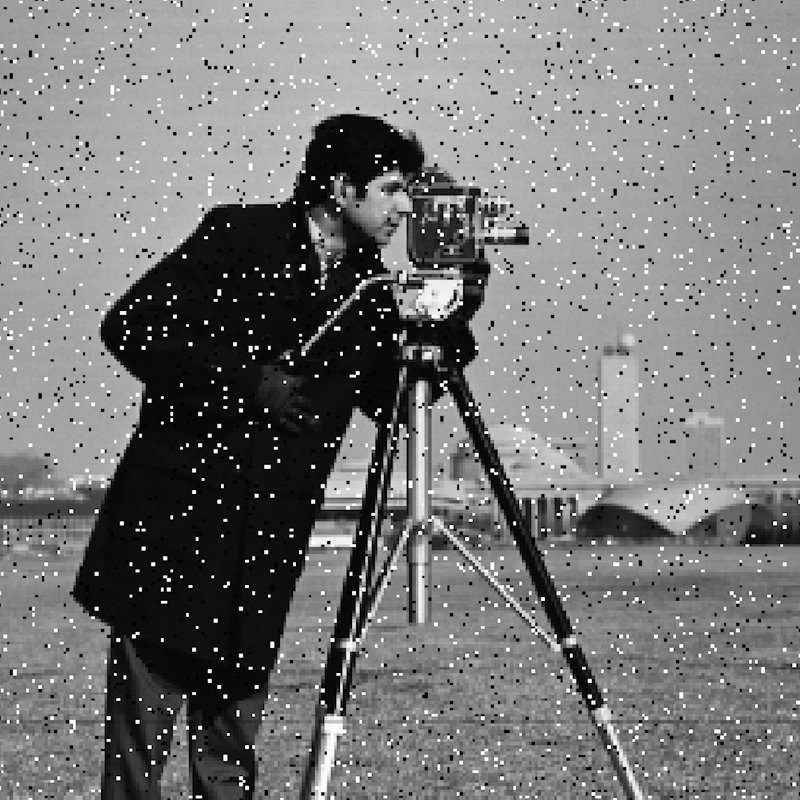
\includegraphics[width=0.4\columnwidth]{images/salt_pepper_noise.jpg}
	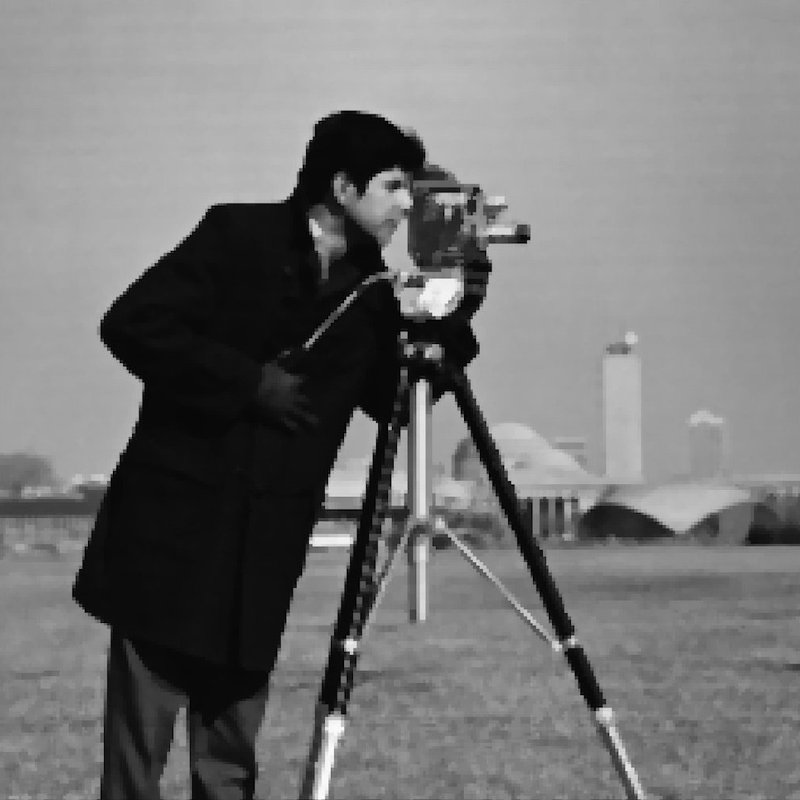
\includegraphics[width=0.4\columnwidth]{images/salt_pepper_median.jpg}
	\caption{Median filter on noise removal: original noisy image (left column), denoised image with median filter (right column).}
	\label{fig:median}
\end{figure}	


Using median filter for noise removal proposes two advantages. First, median is a robust operator where single extreme values in the neighborhood do not affect median value. Secondly, median value is also one actual pixel value of the image so median filter does not create artifacts into the image. For this, median filter is useful in reducing noise of images but still keeping image details and edges. Figure~\ref{fig:median} shows an example of using median filter to remove noise from a noisy cameraman image (first column). From this figure, we can see that median filter greatly reduces salt and pepper noise in the original image (second column).

%%%
\section{Average Filter}

Average filter is also a spatial filter applying to a neighborhood as median filter.  However, the main goal of mean filter is to remove pixel values which are unrepresentative for their surroundings. Average filter is also a linear filter as a convolution. This means that each pixel value is replaced by the average of itself and its neighbors. As other convolution filters, average filter is also based on a kernel, which presents size and shape of the neighborhood to be sampled when computing the mean. The formula of the average filter is given by:

\begin{equation}
k(u,v) = \frac{1}{M} \sum_{(p,q) \in N} i(p,q)
\end{equation}

Where $k(u,v)$ is new pixel value at position $(u,v)$ of the image, $N$ is neighborhood size, $M$ is total number of pixels in the neighborhood $N$, $i(p,q)$ are original pixel values of the image in the neighborhood $N$. 

%%%
\begin{table*}[tb]
	\caption{Example of Average Filter} 
	\label{tab:average_filter}

	\begin{center}
		3$\times$3 Average Filter \\
		$\dfrac{1}{9}\hspace{0.5em}\begin{tabular}{|c|c|c|}
		\hline 
		1 & 1 & 1 \\ 
		\hline 
		1 & 1 & 1 \\ 
		\hline 
		1 & 1 & 1 \\ 
		\hline 
		\end{tabular}$ 	
	\end{center}

	\begin{center}
		5$\times$5 Average Filter \\
		$\dfrac{1}{25}\hspace{0.5em}\begin{tabular}{|c|c|c|c|c|}
		\hline 
		1 & 1 & 1 & 1 & 1 \\ 
		\hline 
		1 & 1 & 1 & 1 & 1 \\ 
		\hline 
		1 & 1 & 1 & 1 & 1 \\ 
		\hline 
		1 & 1 & 1 & 1 & 1 \\ 
		\hline 
		1 & 1 & 1 & 1 & 1 \\ 
		\hline 
		\end{tabular} $
	\end{center}

	\begin{center}
		7$\times$7 Average Filter \\
		$\dfrac{1}{49}\hspace{0.5em}\begin{tabular}{|c|c|c|c|c|c|c|}
		\hline 
		1 & 1 & 1 & 1 & 1 & 1 & 1 \\ 
		\hline 
		1 & 1 & 1 & 1 & 1 & 1 & 1 \\ 
		\hline 
		1 & 1 & 1 & 1 & 1 & 1 & 1 \\ 
		\hline 
		1 & 1 & 1 & 1 & 1 & 1 & 1 \\ 
		\hline 
		1 & 1 & 1 & 1 & 1 & 1 & 1 \\ 
		\hline 
		1 & 1 & 1 & 1 & 1 & 1 & 1 \\ 
		\hline 
		1 & 1 & 1 & 1 & 1 & 1 & 1 \\ 
		\hline 
	\end{tabular} $
	\end{center}

\end{table*}

%%%
The impact of average filter on noise removal depends on its size. It is often that the size of a filter is chosen to be much smaller than the image size. Table~\ref{tab:average_filter} presents three examples of average filter masks of sizes 3$\times$3, 5$\times$5 and 7$\times$7 respectively. From this table, we see that the average filter has three main characteristics: (1) it is in odd ordered, (2) sum of its all elements is equal to 1, and (3) all elements are the same.

When applying average filter to denoise images, there is a trade-off between noise removal and image feature preservation. Specifically, the bigger size of the average filter results in less noise but produces more blurriness to edges and image details. Figure~\ref{fig:meanfilter2} shows impact of average filter size on removing salt and pepper noise of a noisy cameraman image (first column). From this table, 5$\times$5 average filter (last column) removes more noise than 3$\times$3 average filter, but also makes image edges and details more blurred. Due to this, it is important to choose an appropriate size when applying average filter to remove noise.    

%%%
\begin{figure}[h]
\begin{center}
	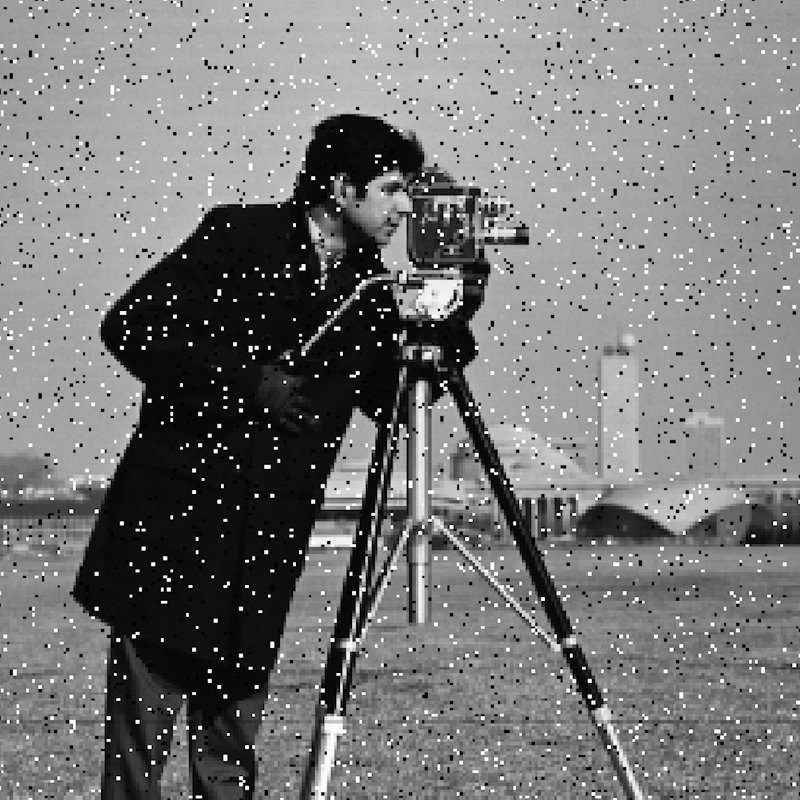
\includegraphics[width=0.3\columnwidth]{images/salt_pepper_noise.jpg}
	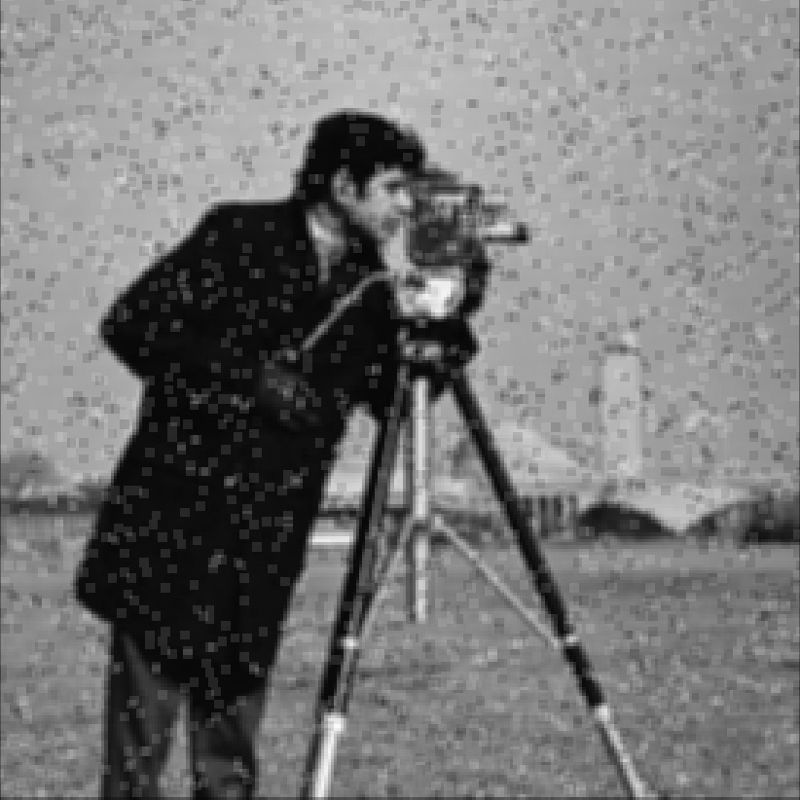
\includegraphics[width=0.3\columnwidth]{images/salt_pepper_average_33.jpg}
	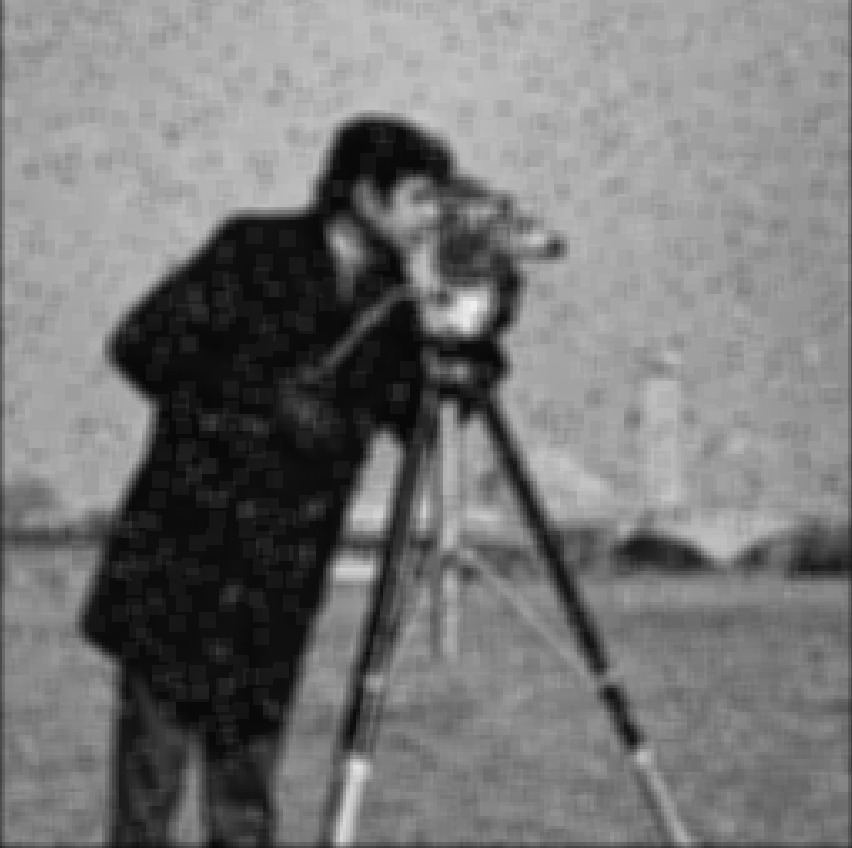
\includegraphics[width=0.3\columnwidth]{images/salt_pepper_average_55.jpg}
	\caption{Impact of average filter size on noise removal: original noisy image (first column), denoised image with 3$\times$3 average filter (second column), denoised image with 5$\times$5 average filter (last column).}	
	\label{fig:meanfilter2}
\end{center}
\end{figure}

%%%
\section{Gaussian Filter}

Gaussian filter is a non-linear filter which performs 2D convolution operator over pixel values so as to blur images or to remove noise and image details. Gaussian filter performs convolution  similarly to average filter, but Gaussian filter uses a different convolution kernel which represents the Gaussian distribution. The formula of 2D Gaussian distribution is given below: 

\begin{equation}
	G(x,y)={\frac {1}{2\pi \sigma ^{2}}}e^{-{\frac {x^{2}+y^{2}}{2\sigma ^{2}}}}
\end{equation}

where $x$ and $y$ are distances from the origin in the horizontal axis and vertical axis respectively, and $\sigma$ is the standard deviation of the 2D Gaussian distribution. The values from this distribution are sampled and used to build a 2D Gaussian convolution matrix using for image blur. Table~\ref{tab:gaussian_filter} presents three examples of gaussian filter masks of sizes 3$\times$3, 5$\times$5 and 7$\times$7 respectively.

In comparison with median filter, gaussian filter is faster in removing noise since multiplying and adding operations is often faster than sorting operations. With mean filter, Gaussian filter is slower but offers better performance of removing noise in frequency domain. This is since mean filter has little ability to separate one band of frequencies from another. 

%%%
\begin{table*}[tb]
	\caption{Example of Gaussian Filters} 
	\label{tab:gaussian_filter}

	\begin{center}
		3$\times$3 Gaussian Filter \\
		$\dfrac{1}{16}\begin{tabular}{|c|c|c|}
		\hline 
		1 & 2 & 1 \\ 
		\hline 
		2 & 4 & 2 \\ 
		\hline 
		1 & 2 & 1 \\ 
		\hline 
		\end{tabular} $
	\end{center}

	\begin{center}
		5$\times$5 Gaussian Filter \\
		$\dfrac{1}{273}\begin{tabular}{|c|c|c|c|c|}
		\hline 
		1 & 4 & 7 & 4 & 1 \\ 
		\hline 
		4 & 16 & 26 & 16 & 4 \\ 
		\hline 
		7 & 26 & 41 & 26 & 7 \\ 
		\hline 
		4 & 16 & 26 & 16 & 4 \\ 
		\hline 
		1 & 4 & 7 & 4 & 1 \\ 
		\hline 
		\end{tabular}$ 
	\end{center}

	\begin{center}
		7$\times$7 Gaussian Filter \\
		$\dfrac{1}{1003}$\begin{tabular}{|c|c|c|c|c|c|c|}
		\hline 
		0 & 0 & 1 & 2 & 1 & 0 & 0 \\ 
		\hline 
		0 & 3 & 13 & 22 & 13 & 3 & 0 \\ 
		\hline 
		1 & 13 & 59 & 97 & 59 & 13 & 1 \\ 
		\hline 
		2 & 22 & 97 & 159 & 97 & 22 & 2 \\ 
		\hline 
		1 & 13 & 59 & 97 & 59 & 13 & 1 \\ 
		\hline 
		0 & 3 & 13 & 22 & 13 & 3 & 0 \\ 
		\hline 
		0 & 0 & 1 & 2 & 1 & 0 & 0 \\ 
		\hline 
		\end{tabular} 
	\end{center}

\end{table*}

%%%
\begin{figure}[tb]
\begin{center}
	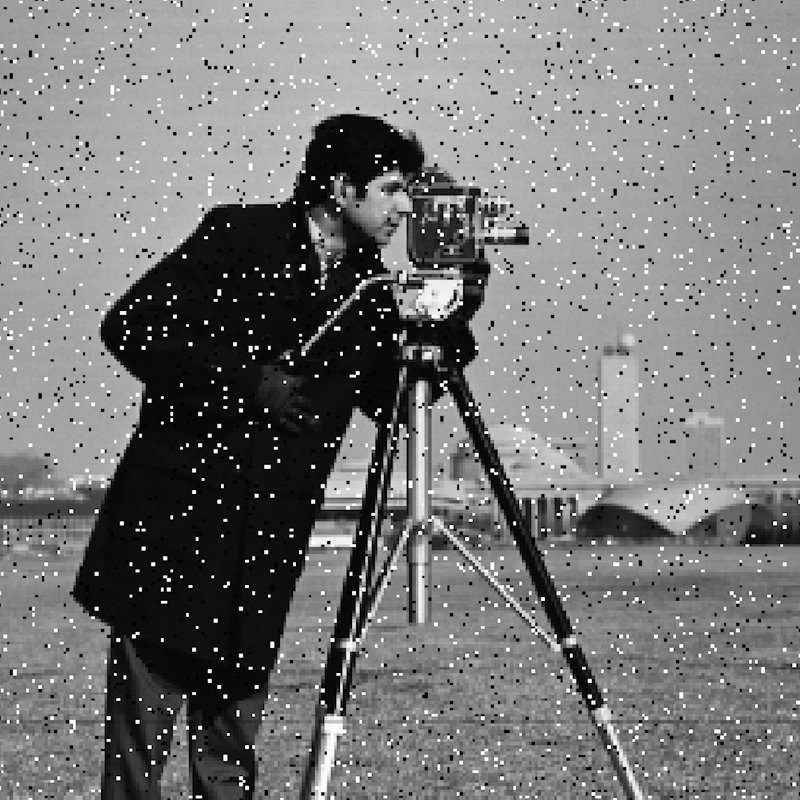
\includegraphics[width=0.4\columnwidth]{images/salt_pepper_noise.jpg}
	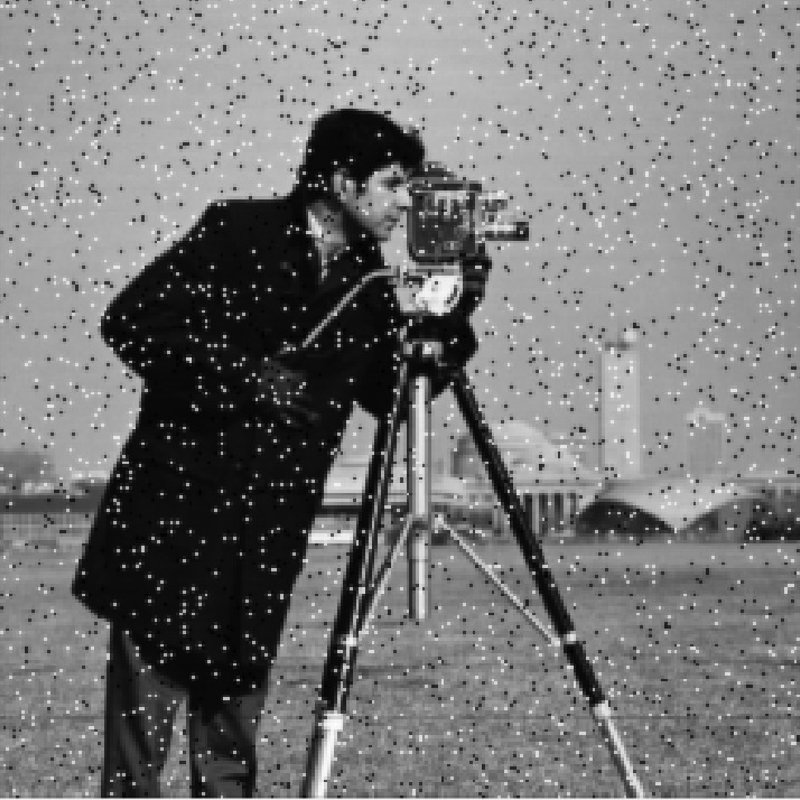
\includegraphics[width=0.4\columnwidth]{images/salt_pepper_gaussian_55.jpg}
	\caption{Gaussian filter on noise removal: original noisy image (first column), denoised image with 5$\times$5 gaussian filter (second column).}	
	\label{fig:gaussianfilter}
\end{center}
\end{figure}

Figure~\ref{fig:gaussianfilter} shows an example of using gaussian filter to remove noise from a noisy cameraman image (first column). From this figure, we can see that gaussian filter reduces noise from the image but also removes the image details and makes it more blurred.

%%%
\section{Wiener Filter}

Weiner filter is a frequency-domain method for image denosing. Wiener filter removes noise from an image signal by minimizing mean square error between the original noiseless image signal and the received image signal. Wiener filter assumes that both signal and noise are stationary linear stochastic processes with known spectral properties.

\begin{comment}
Considering that we need to build a wiener filter in frequency domain as $W(u,v)$, given the received signal $Y(u,v)$ and the denoised image $X(u,v)$. The formula of wiener filter is defined as follows:

\begin{equation}
	\hat{F}(u,v) = \left[ \frac{H^*(u,v) S_f(u,v)}{S_f(u,v) \mid H(u,v) \mid^2 + S_\eta(u,v)} \right] G(u,v)
\end{equation} 
\end{comment}

%%%
\begin{figure}[tb]
\begin{center}
	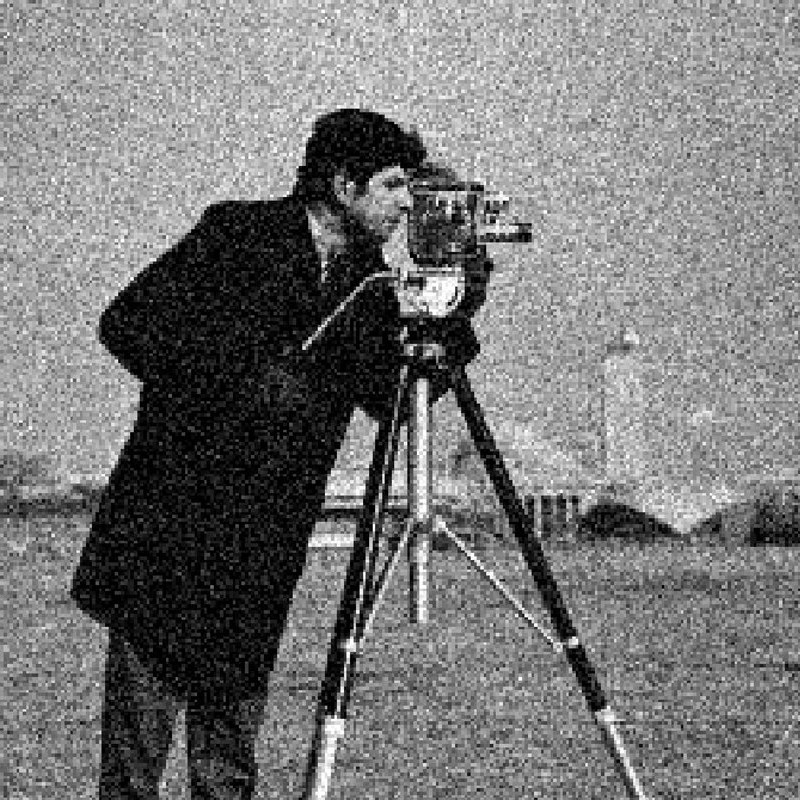
\includegraphics[width=0.4\columnwidth]{images/gaussian_wiener_noise.jpg}
	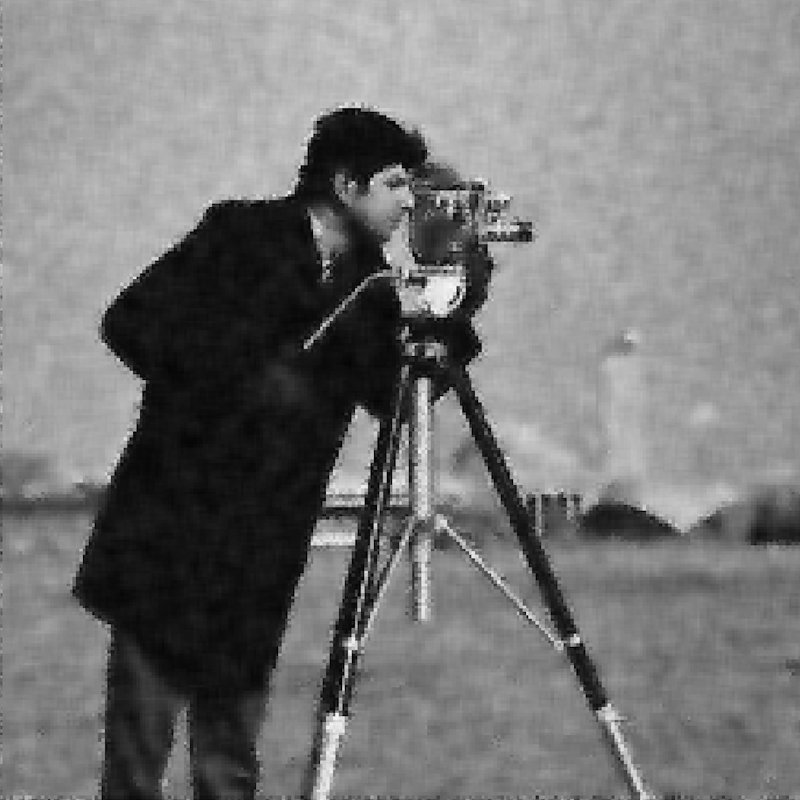
\includegraphics[width=0.4\columnwidth]{images/gaussian_wiener_denoise.jpg}
	\caption{Wiener filter on noise removal: image with gaussian noise (first column), denoised image with 5$\times$5 wiener filter (second column).}	
	\label{fig:wienerfilter}
\end{center}
\end{figure}

Figure~\ref{fig:wienerfilter} shows an example of using wiener filter to remove noise from a noisy cameraman image with additive gaussian noise (first column). From this figure, we can see that wiener filter reduces noise from the image but also makes it more blur.


% TODO: expand this part.
% Estimate of the signal